\providecommand{\main}{..}
\documentclass[\main/notes.tex]{subfiles}

\begin{document}
	\chapter{Graphics Systems and Models}
		\begin{definition}{Computer Graphics}
			All aspects of producing pictures or images using a computer.

			Began 50 years ago, with the display of lines on a \concept{cathode-ray tube (CRT)}.
		\end{definition}

		\begin{definition}{WebGL}
			A graphics software system supported by most modern web browsers.
			A version of \concept{OpenGL} -- the widely accepted standard for
			developing graphics applications.
		\end{definition}

		\section{Applications of Computer Graphics}
			\begin{sidenote}{Four Major Areas}
				\begin{center}
					\begin{enumerate*}[itemjoin=\quad]
						\item Display of information
						\item Design
						\item Simulation and animation
						\item User interface
					\end{enumerate*}
				\end{center}
			\end{sidenote}

			\subsection{Display of Information}
				\begin{example}[Types]
					\begin{itemize}[nosep]
						\item Floor plans
						\item Maps
						\item Statistics Plots
						\item Medical Imaging\\
							\begin{itemize*}[itemjoin=\quad]
								\item Computed Tomography (CT)
								\item Magnetic Resonance Imaging (MRI)
								\item Ultrasound
								\item Positron-emission tomography (PET)
							\end{itemize*}
						\item Scientific visualization
					\end{itemize}
				\end{example}
			\pagebreak

			\subsection{Design}
				Starting with a set of specifications, engines and architects seek a cost-effective
				and aesthetic solution that satisfies the specifications.
				Design is an iterative process.

				Design problems are either \concept{overdetermined} or \concept{underdetermined}.
				\begin{description}[nosep]
					\item[Overdetermined] No solution that satisfies all the criteria.
					\item[Underdetermined] Multiple solutions that satisfy all the criteria.
				\end{description}

				Using interactive graphic tools in \concept{computer-aided design (CAD)} occurs in many
				fields.

			\subsection{Simulation and Animation}
				An example is the training of pilots -- using graphical flight simulators increases safety,
				and reduces training expenses.

				The success of simulators led to using computer graphics for animation, as well as VR.

			\subsection{User Interfaces}
				The predominant way of interacting with computers uses a visual paradigm
				that includes windows, icons, menus, and a pointing device.

		\section{A Graphics System}
			\begin{sidenote}{Six Major Elements in a Graphics System}
				\vspace*{-0.5cm}
				\begin{multicols}{2}
					\begin{enumerate}[nosep]
						\item Input devices
						\item Central Processing Unit
						\item Graphics Processing Unit
						\item Memory
						\item Framebuffer
						\item Output devices
					\end{enumerate}
				\end{multicols}
			\end{sidenote}

			\subsection{Pixels and the Framebuffer}
				\begin{itemize}[nosep]
					\item Virtually all modern graphics systems are \concept{raster-based}.
					\item The image seen on the output device is an array -- the \concept{raster}
					-- of picture elements (\concept{pixels}), produced by the graphics system.
					\item Each pixel corresponds to a location in the image.
					\item The pixels are stored in a part of memory called the \concept{framebuffer}.
				\end{itemize}

				\begin{definition}{Framebuffer Properties}
					\begin{description}
						\item[Resolution] The number of pixels in the framebuffer.
						Determines the detail that can be seen in the image.
						\item[Depth (Precision)] The number of bits used for each pixel.
						Determines properties such as how many colors can be represented on a given system.
						For example, a 1-bit deep framebuffer would allow only two colors,
						whereas an 8-bit deep one would allow $2^8$ (256) colors.
					\end{description}
				\end{definition}

				\begin{sidenote}{Color Systems}
					\begin{description}
						\item[Full-color systems] 24 (or more) bits per pixel.
						These systems can display sufficient colors to represent most images realistically.
						These are also called \concept{true-color} systems, or \concept{RGB color} systems,
						because individual groups of bits in each pixel are assigned to each of the primary
						colors -- red, green, and blue -- that are used in most displays.
						\item[High dynamic range (HDR) systems] 12 or more bits for each color component
						(as opposed to the 8 above).
					\end{description}
				\end{sidenote}

				Until recently, framebuffers stored colors in integer formats.
				More recently, floating point has been used, which allows easier support for HDR.

				In a simple system, the framebuffer holds only the colored pixels displayed on the screen.
				However, in most systems, the framebuffer holds far more information, such as depth
				information.
				In these systems, the framebuffer contains multiple buffers, one of which is the
				\concept{color buffer}.

			\subsection{The CPU and GPU}
				In simple systems, there is a single processor, the \concept{central processing unit (CPU)},
				that performs both normal and graphical processing.
				The main graphical function of the processor is to take specifications of graphical
				primitives generated by application programs,
				and to assign values to the pixels in the framebuffer that best represent these entities.

				\begin{definition}{Rasterization}
					Also called \concept{scan conversion}.
					The conversion of geometric entities to pixel colors and locations in the framebuffer.

					\begin{example}[Triangle Rasterization]
						A triangle is specified by three vertices,
						but to display its outline by the three line segments connecting the vertices,
						the graphics system must generate a set of pixels that appear as line segments to the
						viewer.
					\end{example}
				\end{definition}

				In early graphics systems, the framebuffer was part of the standard memory
				that could be directly addressed by the CPU.

				Nowadays, virtually all graphics systems are characterized by special purpose
				\concept{graphics processing units (GPUs)} that are custom-tailored
				to carry out specific graphics functions.
				The GPU can be located on the motherboard, or on a graphics card.
				The framebuffer is accessed through the GPU and is usually on the same circuit board
				as the GPU.
			\pagebreak

			\subsection{Output Devices}
				\begin{wrapfigure}{r}{0.5\textwidth}
					\begin{center}
						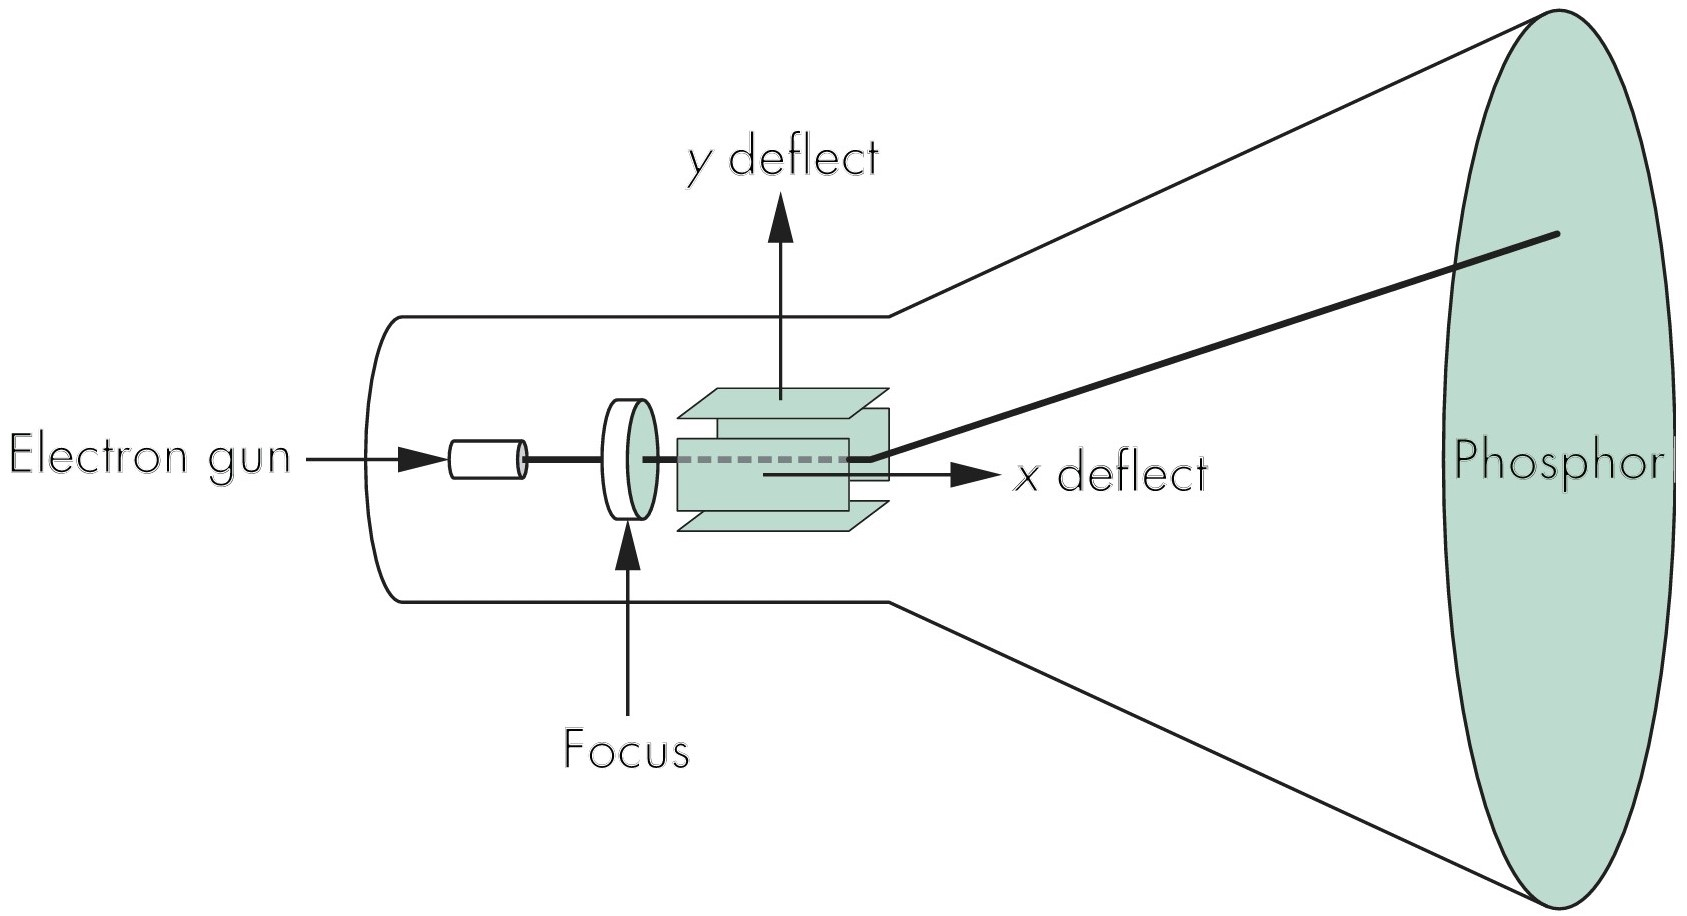
\includegraphics[width=0.48\textwidth]{\main/images/chapter01/cathode_ray_tube.jpg}
					\end{center}
					\caption{Cathode-Ray Tube (CRT)}
				\end{wrapfigure}

				Until recently, the dominant type of display (or \concept{monitor}) was the
				\concept{cathode-ray tube (CRT)}.

				When electrons strike the phosphor coating on the tube, light is emitted.
				The direction of the beam is controlled by two pairs of deflection plates.

				The output of the computer is converted, by digital-to-analog converters,
				to voltages across the $x$ and $y$ deflection plates.
				Light appears on the surface of the CRT when a sufficiently intense beam of electrons
				is directed at the phosphor.

				A typical CRT emits light for a short time -- usually a few milliseconds
				-- after the phosphor is excited by the electron beam.
				For a human to see a steady, flicker-free image, the same path must be \concept{refreshed},
				by the beam at a sufficiently high rate, called the \concept{refresh rate}.
				In older systems, the refresh rate was determined by the frequency of the power system:
				60 Hz in the US, and 50 Hz in much of the rest of the world.

				\begin{definition}{Vector CRT}
					If the voltages steering the beam change at a constant rate,
					the beam will trace a straight line, visible to the viewer.
					This is called the \mbox{\concept{random-scan}}, \concept{calligraphic},
					or \concept{vector} CRT,
					because the beam can be moved directly from any position to any other position.
					This is the basis of early graphics systems that predated the present raster technology.
				\end{definition}

				\begin{definition}{Raster CRT}
					In a raster system, the graphics system takes pixels from the framebuffer and
					displays them as points on the surface of the display in one of two ways:
					\begin{descriptimize}[nosep]
						\item[Noninterlaced] Pixels are displayed row by row,
						or scan line by scan line, at the refresh rate.
						\item[Interlaced] Odd rows and even rows are refreshed alternately.
						Used in commercial television.
						If the display is operating at 60 Hz, the screen is redrawn only 30 times per second.
					\end{descriptimize}
				\end{definition}

				Color CRTs have three different-colored phosphors (red, green, and blue),
				arranged in small groups.
				A common style is to arrange them in triangular groups called \concept{triads},
				where each triad consists of three phosphors: one for each primary color.
				Most color CRTs have three electron beams, corresponding to the types of phosphors.

				In the shadow-mask CRT, a metal screen with small holes (the \concept{shadow-mask})
				ensures that an electron beam excites only phosphors of the proper color.

				CRTs are still common display devices, but are being replaced by flat-screen technologies.
				Flat-panel monitors are inherently raster-based.
				All technologies available -- including light-emitting diodes (LEDs),
				liquid-crystal displays (LCD's), and plasma panels --
				use a two-dimensional grid to address individual light-emitting elements.
				\pagebreak

				\begin{wrapfigure}{l}{0.5\textwidth}
					\begin{center}
						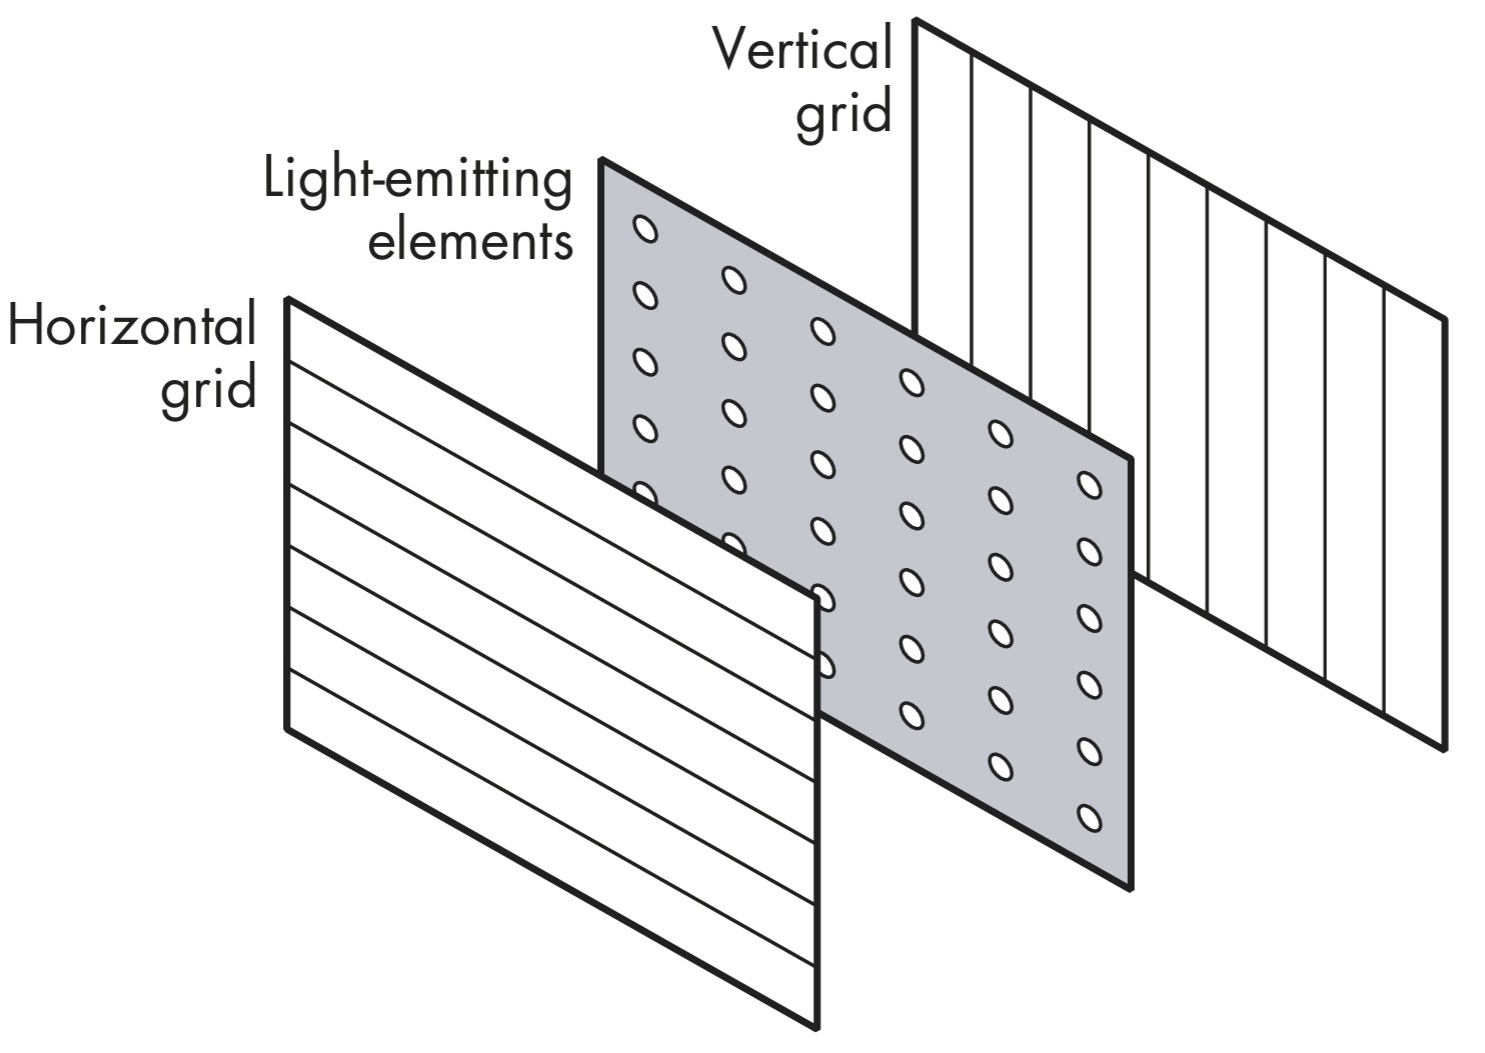
\includegraphics[width=0.48\textwidth]{\main/images/chapter01/flat_panel_display.jpg}
					\end{center}
					\caption{Generic Flat-Panel Display}
				\end{wrapfigure}

				A flat-panel display works as follows:

				The two outside plates each contain parallel grids of wires that are oriented perpendicular
				to each other.
				By sending electrical signals to the proper wire in each grid,
				the electrical field at the intersection of the two wires
				can be made strong enough to control the corresponding element in the middle plate.

				The middle plate in an LED panel contains light-emitting diodes
				that can be turned on and off by the electrical signals sent on the grid.
				In an LCD, the electrical field controls the polarization of the liquid crystals in
				the middle panel,
				thus turning on and off light passing through the panel.
				A plasma panel uses the voltages on the grids to energize gases embedded between the
				glass panels holding the grids.
				The energized gas becomes a glowing plasma.

				Most projection systems are raster-based.
				They use a variety of technologies including CRTs and digital light projection (DLP).
				These systems act as standard monitors with similar resolutions and perspectives.
				Hard-copy devices, such as printers and plotters, are also raster-based, but cannot be
				refreshed.

				Stereo (3D) television displays use alternate refresh cycles to switch the display 
				between an image for the left eye and an image for the right eye.
				The viewer wears special glasses that are coupled to the refresh cycle.

			\subsection{Input Devices}
				Most graphics systems provide a keyboard and at least one other input device.
				The most common input devices are the mouse, the joystick, and the data tablet.
				Each of these provides positional information to the system,
				and is usually equipped with one or more buttons to provide signals to the processor.
				These devices are often called \concept{pointing devices},
				and allow a user to indicate a particular location on the display.

				Due to new input devices appearing regularly,
				our graphics programs should implement a flexible model for incorporating input devices.

\end{document}